%!TEX root = paper.tex
\section{Evaluation}
\label{sec:eval}

\begin{figure*}
\centering
    \subfigure[LDA]{
        \label{fig:exp_lda}
        %\includegraphics[width=0.3\linewidth]{figures/fig_10B17_case1}
        \includegraphics[width=0.3\linewidth]{figs/exp_lda.eps}
    }
    \subfigure[SLDA]{
        \label{fig:exp_slda}
        %\includegraphics[width=0.3\linewidth]{figures/fig_15B31_case2}
        \includegraphics[width=0.3\linewidth]{figs/exp_slda.eps}
    }
    \subfigure[DCMLDA]{
        \label{fig:exp_dcmlda}
        %\includegraphics[width=0.3\linewidth]{figures/fig_48B48_case6}
        \includegraphics[width=0.3\linewidth]{figs/exp_dcmlda.eps}
    }
	\caption{Running Time}
    \label{fig:exp_comparison}
\end{figure*} 

In this section, we present performance evaluation of InferSpark, based on constructing 
and carrying out statistic inference on three models: Latent Dirichlet Allocation (LDA), Sentence-LDA (SLDA) \cite{Jo2011}, and Dirichlet Compound Multinomial LDA (DCMLDA) \cite{Doyle2009}.
LDA is a standard model in topic modeling, which takes in a collection of documents
and infers the topics of the documents.  
Sentence-LDA (SLDA) is a model for finding aspects in online reviews, which takes in online reviews, and infers the aspects.
Dirichlet Compound Multinomial LDA (DCMLDA) is another topic model that accounts for burstiness in documents.
All models can be implemented in InferSpark using less than 9 lines of code (see \figref{fig:intro_lda_def} and Appendix \ref{models}).
For comparison, we include MLlib in our study whenever applicable.
MLlib includes LDA as standard models.  However, MLlib does not include SLDA and DCMLDA.
There are other probabilistic programming frameworks apart from Infer.NET (see Section \ref{sec:related}).
All of them are unable to scale-out onto multiple machines yet.  
Infer.NET so far is the most predominant one with the best performance, so we also include it in our study whenever applicable.

All the experiments are done on nodes running Linux with 2.6GHz quad-core, 32GB memory, and 700GB hard disk. 
Spark 1.4.1 with scala 2.11.6 is installed on all nodes.
The default cluster size for InferSpark and MLlib is 24 data nodes and 1 master node.
Infer.NET can only use one such node.
The data for running LDA, SLDA, and DCMLDA are listed in Table \ref{data}.
The wikipedia dataset is the wikidump. Amazon is a dataset of Amazon reviews
used in \cite{Jo2011}.
We run 50 iterations and do checkpointing every 10 iterations for each model on each dataset.

\begin{table}\scriptsize
\caption{Datasets}
\label{data}
\begin{tabular}{ccc}
     \begin{tabular}{|c|c|c|}     \hline
        {Wikipedia} & words & topics \\\hline\hline
         0.2\% & 541,644 & 96 \\\hline
         0.5\% & 1,324,816  & 96 \\         \hline
         \multicolumn{3}{c}{LDA} \\
     \end{tabular}
          &
     \begin{tabular}{|c|c|c|}     \hline
        {Amazon} & words & topics \\\hline\hline
         6\% & 349,569 & 96 \\\hline
         10\% & 607,430  & 96 \\         \hline
         \multicolumn{3}{c}{SLDA} \\
     \end{tabular}
     \\\\
     \multicolumn{2}{c}{
     \begin{tabular}{|c|c|c|}     \hline
        {Wikipedia} & words & topics \\\hline\hline
         0.5\% & 1,324,816 & 10 \\\hline
         1\% & 2,596,155  & 10 \\         \hline
         \multicolumn{3}{c}{DCMLDA} \\
     \end{tabular}
     }
\end{tabular}
\end{table}

\subsection{Overall Performance}


\figref{fig:exp_comparison} shows the time of running LDA, SLDA, and DCMLDA 
on InferSpark, Infer.NET, and MLlib.
Infer.NET cannot finish the inference tasks on all three models within a week.
MLlib supports only LDA, and is more efficient than InferSpark in that case.
However, we remark that MLlib uses the EM algorithm which only
calculates Maximum A Posterior instead of the full posterior and is specific to LDA.
In contrast, InferSpark aims to provide a handy programming platform for statistician and domain users to build and test various customized models based on big data.
It would not be possible to be done by any current probabilistic frameworks nor with Spark/GraphX directly unless huge programming effort is devoted.  
MLlib versus InferSpark 
is similar to C++ programs versus DBMS: highly optimized C++ programs are more efficient, 
but DBMS achieves good performance with lower development time.
From now on, we focus on evaluating the performance of InferSpark.



Table \ref{breakdown} shows the time breakdown of InferSpark.
The inference process executed by GraphX, as expected, dominates the running time.
The MPG construction step executed by Spark, can finish within two minutes.
The Bayesian network construction and code generation can be done in seconds.


\begin{table*}
\caption{Time Breakdown (in seconds and \%)}
\label{breakdown}
\begin{tabular}{|l||*{8}{r|}r|}
\hline
Model & \multicolumn{2}{c|}{B.N. Construction} & \multicolumn{2}{c|}{Code Generation}	& \multicolumn{4}{c|}{Execution} & Total \\\cline{6-9} 
  & \multicolumn{2}{c|}{ } & \multicolumn{2}{c|}{ }	& \multicolumn{2}{c|}{MPG Construction} & \multicolumn{2}{c|}{Inference} &	 \\ \hline \hline
LDA 541644 words	& 21.911	& 1.34\%	& 11.15 &	0.68\%	& 38.147	& 2.33\% &	1566.692 & 95.65\%	& 1637.9 \\ \hline
LDA 1324816 words &	21.911 & 0.70\% & 12.25	& 0.39\% & 79.4 & 2.55\%	& 3002.1 & 96.36\% &	3115.661 \\ \hline
SLDA 349569 words &	21.867 & 1.76\% & 11.05 &	0.89\%	& 26.33 & 2.12\% &	1182.2	& 95.23\%	& 1241.447 \\ \hline
SLDA 607430 words & 21.867 & 0.96\%	& 11.69	& 0.52\% & 41.152	& 1.81\%	& 2193.391	& 96.71\%	& 2268.1 \\ \hline
DCMLDA 1324816 words & 22.658 & 0.65\%	& 10.52 & 0.30\% &	20.923	& 0.60\% & 3448.699	& 98.46\% &	3502.8 \\ \hline
DCMLDA 2596155 words & 22.658 & 0.28\% & 11.55 & 0.14\%	& 39.549 & 0.48\%	& 8153.969 & 99.10\%	& 8227.726 \\ \hline

\end{tabular}
\end{table*} 





\subsection{Scaling-Up}

\figref{fig:scale-up} shows the total running time of LDA, SLDA, and DCMLDA on InferSpark
by scaling the data size (in words).
InferSpark scales well with the data size.
DCMLDA exhibits even super-linear scale-up. This is because as the data size goes up, 
the probability of selecting larger documents goes up. Consequently,
the growth in the total number of random variables is less than proportional, which gives rise
to the super-linearity.

\begin{figure}[h]\centering
	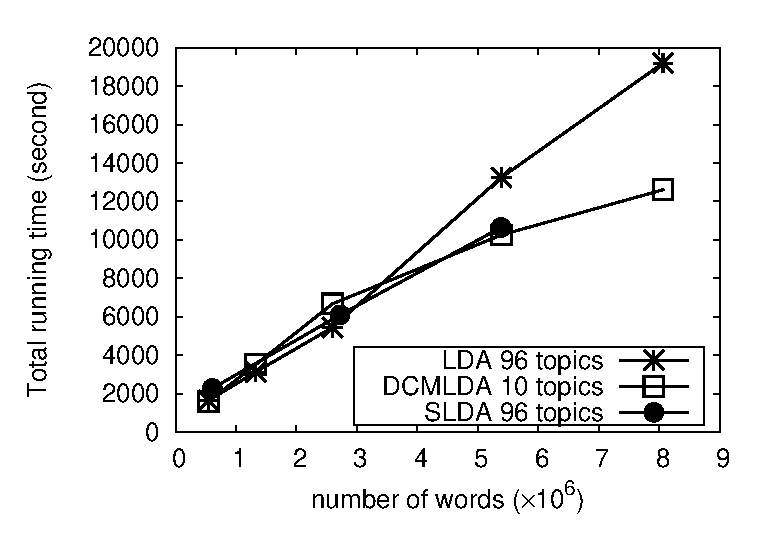
\includegraphics[width=0.35\textwidth]{figs/exp_lda_datasize.eps}
	\caption{Scaling-up}
	\label{fig:scale-up}
\end{figure}



\subsection{Scaling-Out}

\figref{fig:scale-out} shows the total running time of LDA on InferSpark in
different cluster sizes. For each model, we use fixed size of dataset.  DCMLDA
and LDA both use the 2\% Wikipedia dataset. SLDA uses the 50\% amazon dataset.
We observe that InferSpark can achieve linear scale-out. 

\begin{figure}[h]
	\centering
	\includegraphics[width=0.35\textwidth]{figs/exp_clustersize.eps}
	\caption{Scaling-out}
	\label{fig:scale-out}
\end{figure}


\subsection{Partitioning Strategy}

\figref{fig:exp_partition_strategy} shows the running time of LDA(0.2\% Wikipedia dataset, 96 topics) on InferSpark
using our partitioning strategy  and 
GraphX partitioning strategies: 
EdgePartition2D  (2D)
RandomVertexCut (RVC),
CanonicalRandomVertexCut (CRVC), and
EdgePartition1D (1D).
We observe that the running time is propotional to the size of EdgeRDD.
Our partition strategy yields the best performance for running VMP on the
message passing graphs.  Our analysis shows that RVC and CRVC should have the
same results. The slight difference in the figure is caused by the randomness
of different hash functions.



%\begin{figure*}[!ht]
%	\tiny
%\begin{tabular}{|*{6}{l|}}
%	\hline
%	Experiement & Compilation (s) & Graph Building (s) & First Iteration (s) & Non-checkpointing iteration (s) & checkpointing iteration (s) \\\hline
%	LDA 2596155 words & 9.2 & 139.6 & 102.4 & 91.4 & 236.6 \\\hline
%	LDA 5386900 words & 9.1 & 302.8 & 309.8 & 226.2 & 555.2 \\\hline
%	LDA 8062163 words & 11.8 & 415.2 & 330.4 & 301.6 & 1050.4 \\\hline
%	SLDA 349569 words & 9.8 & 26.8 & 24.9 & 20.9 & 50.8 \\\hline
%	SLDA 607430 words & 10.4 & 41.8 & 42.8 & 38.6 & 94.5 \\\hline
%	DCMLDA 282660 words 96 topics & 11.0 & 29.9 & 163.1 & 141.4 & 336.0 \\\hline
%	DCMLDA 2596155 words 10 topics & 10.6 & 40.0 & 251.5 & 179.6 & 381.4 \\\hline
%\end{tabular}
%\caption{Time Breakdown (\%) of InferSpark (a) BN Construction; (b) Code Generation; (c) GraphX Inference}
%\label{fig:exp_times}
%\end{figure*}

%\begin{figure}[h]
%	\includegraphics[width=0.45\textwidth]{figs/exp_lda.eps}
%	\caption{Comprison of Average Iteration Time of LDA}
%	\label{fig:exp_lda}
%\end{figure}
%
%\begin{figure}[h]
%	\includegraphics[width=0.45\textwidth]{figs/exp_slda.eps}
%	\caption{Comprison of Average Iteration Time of Sentence-LDA}
%	\label{fig:exp_slda}
%\end{figure}
%
%\begin{figure}[h]
%	\includegraphics[width=0.45\textwidth]{figs/exp_dcmlda.eps}
%	\caption{Comparison of Average Iteration Time of Dirichlet Compound Multinomial LDA}
%	\label{fig:exp_dcmlda}
%\end{figure}



%\begin{figure}[h]
%	\includegraphics[width=0.45\textwidth]{figs/exp_slda_datasize.eps}
%	\caption{Inferspark Average Iteration Time vs Datasize of SLDA}
%	\label{fig:exp_slda_datasize}
%\end{figure}

\begin{figure}[h]\centering
	\includegraphics[width=0.35\textwidth]{figs/exp_partition_strategy.eps}
	\caption{Comparison of Different Partition Strategies}
	\label{fig:exp_partition_strategy}
\end{figure}


